\documentclass{article}\usepackage[]{graphicx}\usepackage[]{xcolor}
% maxwidth is the original width if it is less than linewidth
% otherwise use linewidth (to make sure the graphics do not exceed the margin)
\makeatletter
\def\maxwidth{ %
  \ifdim\Gin@nat@width>\linewidth
    \linewidth
  \else
    \Gin@nat@width
  \fi
}
\makeatother

\definecolor{fgcolor}{rgb}{0.345, 0.345, 0.345}
\newcommand{\hlnum}[1]{\textcolor[rgb]{0.686,0.059,0.569}{#1}}%
\newcommand{\hlsng}[1]{\textcolor[rgb]{0.192,0.494,0.8}{#1}}%
\newcommand{\hlcom}[1]{\textcolor[rgb]{0.678,0.584,0.686}{\textit{#1}}}%
\newcommand{\hlopt}[1]{\textcolor[rgb]{0,0,0}{#1}}%
\newcommand{\hldef}[1]{\textcolor[rgb]{0.345,0.345,0.345}{#1}}%
\newcommand{\hlkwa}[1]{\textcolor[rgb]{0.161,0.373,0.58}{\textbf{#1}}}%
\newcommand{\hlkwb}[1]{\textcolor[rgb]{0.69,0.353,0.396}{#1}}%
\newcommand{\hlkwc}[1]{\textcolor[rgb]{0.333,0.667,0.333}{#1}}%
\newcommand{\hlkwd}[1]{\textcolor[rgb]{0.737,0.353,0.396}{\textbf{#1}}}%
\let\hlipl\hlkwb

\usepackage{framed}
\makeatletter
\newenvironment{kframe}{%
 \def\at@end@of@kframe{}%
 \ifinner\ifhmode%
  \def\at@end@of@kframe{\end{minipage}}%
  \begin{minipage}{\columnwidth}%
 \fi\fi%
 \def\FrameCommand##1{\hskip\@totalleftmargin \hskip-\fboxsep
 \colorbox{shadecolor}{##1}\hskip-\fboxsep
     % There is no \\@totalrightmargin, so:
     \hskip-\linewidth \hskip-\@totalleftmargin \hskip\columnwidth}%
 \MakeFramed {\advance\hsize-\width
   \@totalleftmargin\z@ \linewidth\hsize
   \@setminipage}}%
 {\par\unskip\endMakeFramed%
 \at@end@of@kframe}
\makeatother

\definecolor{shadecolor}{rgb}{.97, .97, .97}
\definecolor{messagecolor}{rgb}{0, 0, 0}
\definecolor{warningcolor}{rgb}{1, 0, 1}
\definecolor{errorcolor}{rgb}{1, 0, 0}
\newenvironment{knitrout}{}{} % an empty environment to be redefined in TeX

\usepackage{alltt}
\usepackage{amsmath} %This allows me to use the align functionality.
                     %If you find yourself trying to replicate
                     %something you found online, ensure you're
                     %loading the necessary packages!
\usepackage{amsfonts}%Math font
\usepackage{graphicx}%For including graphics
\usepackage{hyperref}%For Hyperlinks
\usepackage[shortlabels]{enumitem}% For enumerated lists with labels specified
                                  % We had to run tlmgr_install("enumitem") in R
\hypersetup{colorlinks = true,citecolor=black} %set citations to have black (not green) color
\usepackage{natbib}        %For the bibliography
\setlength{\bibsep}{0pt plus 0.3ex}
\bibliographystyle{apalike}%For the bibliography
\usepackage[margin=0.50in]{geometry}
\usepackage{float}
\usepackage{multicol}

%fix for figures
\usepackage{caption}
\newenvironment{Figure}
  {\par\medskip\noindent\minipage{\linewidth}}
  {\endminipage\par\medskip}
\IfFileExists{upquote.sty}{\usepackage{upquote}}{}
\begin{document}

\vspace{-1in}
\title{Lab 10 -- MATH 240 -- Computational Statistics}

\author{
  Sankalp Ojha \\
  Colgate University  \\
  Mathematics  \\
  {\tt sojha@colgate.edu}
}

\date{04/10/2025}

\maketitle

\begin{multicols}{2}
%\raggedcolumns % If your spacing gets messed up try uncommenting 
                % this line
\begin{abstract}
In this lab, we analyzed the validity of statements made by the Gallup survey. The Gallup survey states that a sample size of 1004 should produce a 4\% MOE and doubling the sample size should halve the MOE. Both statements were found to be false through the various simulations ran in this lab.
\end{abstract}

\noindent \textbf{Keywords:} Margin Of Error (MOE), Estimated Margin Of Error, Wilson Estimate, Sample Size, and Proportion.

\section{Introduction}
Gallup polls published a document called \textit{“How Are Polls Conducted?”} that describes how Gallup selects people to include in its poll and other details. Gallup states towards the end of the document:
\\
\\
\textit{“For example, with a sample size of 1,000 national adults (derived using careful random selection procedures), the results are highly likely to be accurate within a margin of error of ±4 percentage points.”
\\
\\
“If Gallup increases a poll sample size to 2,000, the results would then be accurate within ±2%
of the underlying population value, a gain of two percentage points in terms of accuracy, but with a 100\% increase in the cost of conducting the survey.”}

In a study from February 3-16, 2025 poll of 1,004 adults aged 18+ living in all 50 U.S. states and the District of Columbia showed that only 39\% of Americans were satisfied with the United States's position in the world, whereas 59\% of people were dissatisfied. \textbf{Note:} 2\% had no opinion on the United States's position. Gallup reported the ±4\% margin of error.

Through this lab, we aim to study how larger sample sizes lead to lowering the margin of error. Margin of error is a measure which aims to describe the variation in our using the sample proportion $\hat{p}$ as an estimate of \textit{p}. The measure aims to tell us how much the sample proportion to differ from the proportion for the entire population.

Statisticians and quantitative researchers aim to report their studies with at least 95\% confidence. Having a 95\% confidence indicates that the researcher is 95\% confident that if we conduct the study repeatedly, the interval would contain the actual proportion 95\% of the time.

For this lab, we first ran simulations of 10K random polls for a sample size of 1004 individuals and again with a sample size of 2008 individuals to analyze whether the statement of Gallup claiming doubling the sample size will decrease the MOE. Both simulations were conducted assuming we had a known probability, \textit{p}, of 0.39. We then used resampling to obtain the MOE and sampling distribution for $\hat{p}$. We finally ran simulations where we varied both the sample size, n, and probability, p, to see how varying combinations of n and p affect the estimated MOE and Wilson MOE.

\section{Simulations}
To conduct our basic and resampling simulations, we need to follow the process of setting a sample size, declaring an amount of polls to randomly conduct, and calculating the MOE for the given data. The Simulation over \textit{n} and \textit{p} and Actual Margin of Error Calculation sections differed as they ran simulations varying both the n, sample size, and p, probability, parameters. To summarize the data from our simulations, we used the \texttt{ggplot2} \citep{ggplot2} and \texttt{patchwork} \citep{patchwork} packages to make and combine the plots.

\subsection{Basic Simulation}
For the basic simulation, we ran a simulation with 10K random polls. We assumed the probability of surveying a satisfied US citizen was 0.39, as giving by the Gallup study. The sample size for the first simulation was $n = 1004$ and $n = 2008$ individuals for the second simulation. We used \texttt{ribom()} to generate our random samples within the constraints.

\subsection{Resampling}
In the previous section, we conducted samples based on an assumed value of p, 0.39. Resampling will allow us to forgo the assumption made about the sample proportion in the previous section and simulate our own sample distribution of $\hat{p}$ for a Gallup survey. \textbf{Note:} The data which can be used for resampling is constrained to the sample size of $n = 1004$. We ran 1000 resamples to find the sample distribution of $\hat{p}$.

\subsection{Simulation over \textit{n} and \textit{p}}
So far the simulations were conducted under a constrained sample size and proportion. The next simulation aims to represent how the MOE varies as the sample size and proportion change for a sample. Using nested \texttt{for} loops with varying sample sizes from 100 to 3000 in increments of 10, proportions from 0.01 to 0.99 in increments of 0.01, and a set poll size of 10K, as in the basic simulation, simulations were ran for each condition and saved to a \texttt{tibble}. The MOE was summarized using a \verb|geom_raster()| plot. 

\subsection{Wilson MOE Calculation}
So far, we had been calculating the MOE by halving the range of the middle 95\%. Now, we turn to the Wilson MOE which is giving by the equation: \[\text{MOE}_{\text{w}} = z_{1-\alpha/2}\frac{ \sqrt{n\hat{p}(1-\hat{p}) + \frac{{z^2_{1-\alpha/2}}}{4}}}{n + {z^2_{1-\alpha/2}}}\]

The simulation for this section was ran the same as for the Simulation over \textit{n} and \textit{p} section, but we used the Wilson MOE equation to calculate the MOE. Once again we used \verb|geom_raster()| to summarize the data showing MOE as a function of n and p. 

\section{Results By Simulation}
\subsection{Basic Simulation Results}
The Basic simulation resulted in an almost Gaussian shape. The first histogram summarizes the sampling distribution for a sample size of $n = 1004$. The bottom histogram summarizes the sampling distribution for a sample size of $n = 2008$. The estimated MOE for the $n = 1004$ sampling distribution is 2.99\%, whereas the estimated MOE for the $n = 2008$ sampling distribution is 2.09\%. As can be seen in the plots, as the sample size increases the distribution tends closer to the defined proportion of 0.39. Through the MOEs it can be seen that Gallup's estimate of a 4\% error for a sample size of $n = 1004$ and 2\% for a sample size of $n = 2008$ are incorrect. Furthermore, doubling the sample size does \textbf{not} halve the MOE, contrary to what Gallup suggested. 

\begin{Figure}
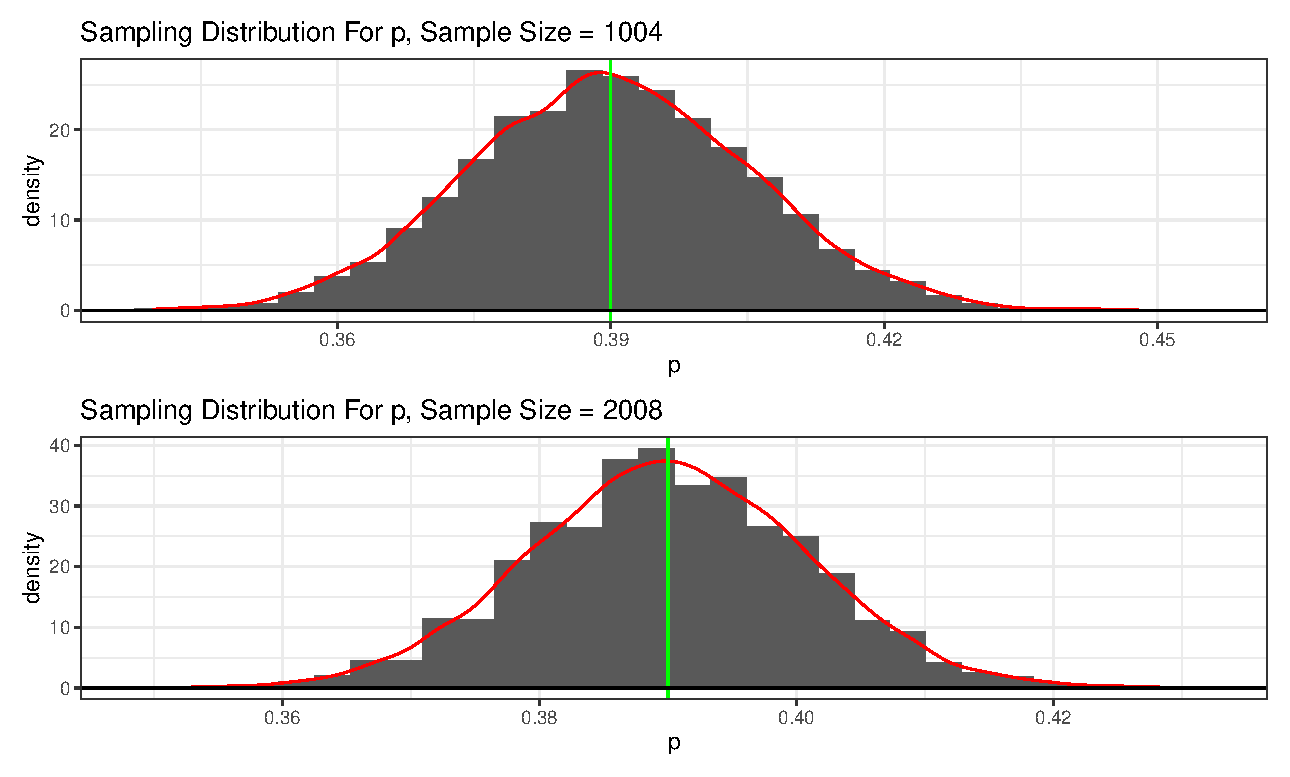
\includegraphics[scale=0.4]{Rplot.pdf}
\captionof{figure}{Plots for Sampling Distribution of $p$}
\label{plot1}
\end{Figure}

\subsection{Resampling Results}
The estimated MOE for sampling distribution of $\hat{p}$ with a sample size of $n = 1004$ is 3.09\%. This is once again not near the 4\% MOE presented by Gallup. The sampling distribution itself is approximately Gaussian. Upon visual inspection, the sampling distribution for $\hat{p}$ is centered at roughly a $\hat{p}$ value of 0.39, which is similar to the proportion used in the Basic Simulation.

\begin{center}
\begin{Figure}
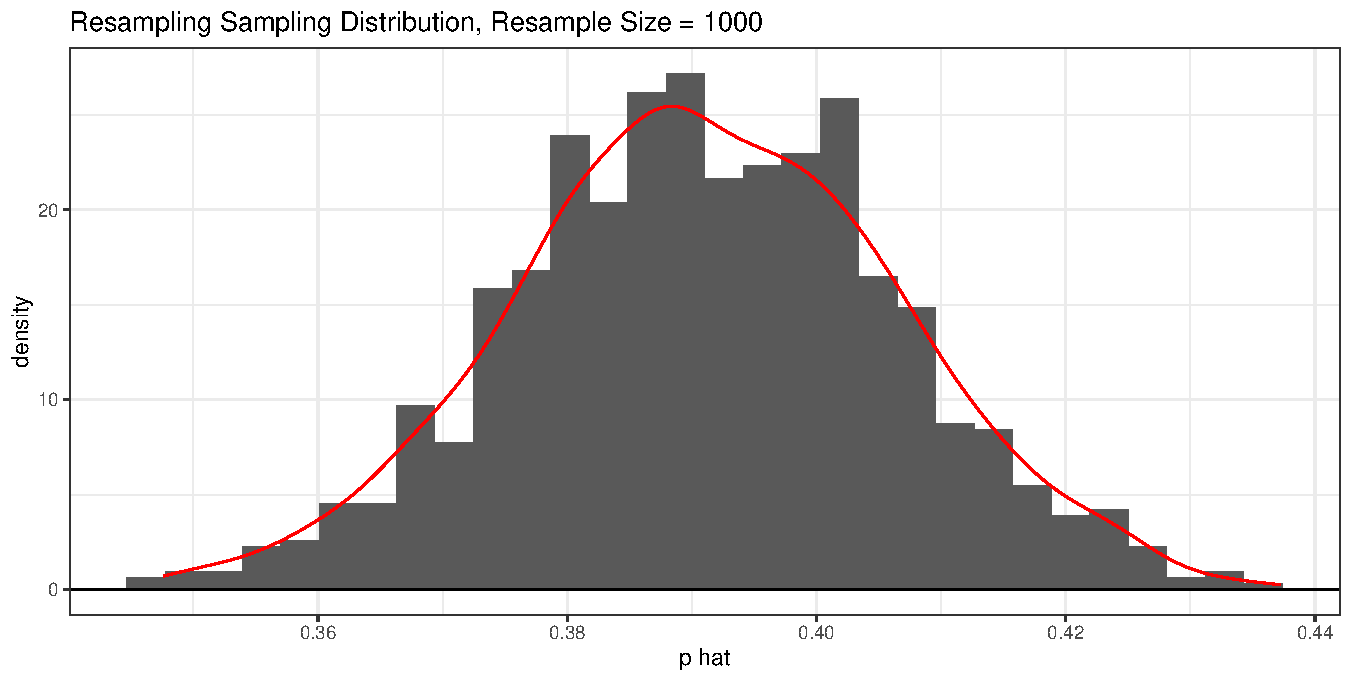
\includegraphics[scale=0.35]{Rplot01.pdf}
\captionof{figure}{Plots for Resampling Sampling Distribution of $\hat{p}$}
\label{plot2}
\end{Figure}
\end{center}

\subsection{\textit{n} and \textit{p} MOE and Wilson MOE Results}
In the appendix, Figure \ref{plot3} shows the \verb|geom_raster()| plot showing the heat map of how n and p affect the estimated MOE (plot on the left) and how n and p affect the Wilson MOE (plot on the right). Both plots look fairly similar and follow a similar gradient as n increases from 100 to 3000. It should be noted that the p seems to be a larger factor which affects both the estimated MOE and Wilson MOE, in comparison to n for lower values of n. As we look across a the plot for a given n, for example $n = 150$, we can notice how the value of p greatly varies the MOEs. The power of large sample sizes can be seen through both plots as larger samples supply more information which lowers ambiguity, MOE values. Through both plots, we can also notice the intersection of $n = 2008$, $n = 1004$, and $p = 0.39$ lines correspond to the MOE values found in the earlier simulations. The final component of the plots which was interesting is that the transition between the various regions is smoother in the Wilson plot, whereas the Estimated plot has portions which are grainy.

\section{Discussion}
Through this lab, it was demonstrated that larger sample sizes lower lead to low MOE calculations and Gallup's statements about how MOE values change with changing the sample size are false. As shown through the \verb|geom_raster()| plots, the MOE calculations approach zero as the sample size increases to 3000. The greater number of samples leads to less ambiguity about the sample. Further the 4\% error mentioned in the Gallup survey did not hold true for our simulations. The second statement about doubling the sample size leads to halved MOE also does not hold. MOE is function of two variables, n and p, so we cannot simply halve the MOE when we double sample size.

%%%%%%%%%%%%%%%%%%%%%%%%%%%%%%%%%%%%%%%%%%%%%%%%%%%%%%%%%%%%%%%%%%%%%%%%%%%%%%%%
% Bibliography
%%%%%%%%%%%%%%%%%%%%%%%%%%%%%%%%%%%%%%%%%%%%%%%%%%%%%%%%%%%%%%%%%%%%%%%%%%%%%%%%
\vspace{2em}
\begin{tiny}
\bibliography{bib8}
\end{tiny}
\end{multicols}

%%%%%%%%%%%%%%%%%%%%%%%%%%%%%%%%%%%%%%%%%%%%%%%%%%%%%%%%%%%%%%%%%%%%%%%%%%%%%%%%
% Appendix
%%%%%%%%%%%%%%%%%%%%%%%%%%%%%%%%%%%%%%%%%%%%%%%%%%%%%%%%%%%%%%%%%%%%%%%%%%%%%%%%
\newpage
\onecolumn
\section{Appendix}

\begin{Figure}
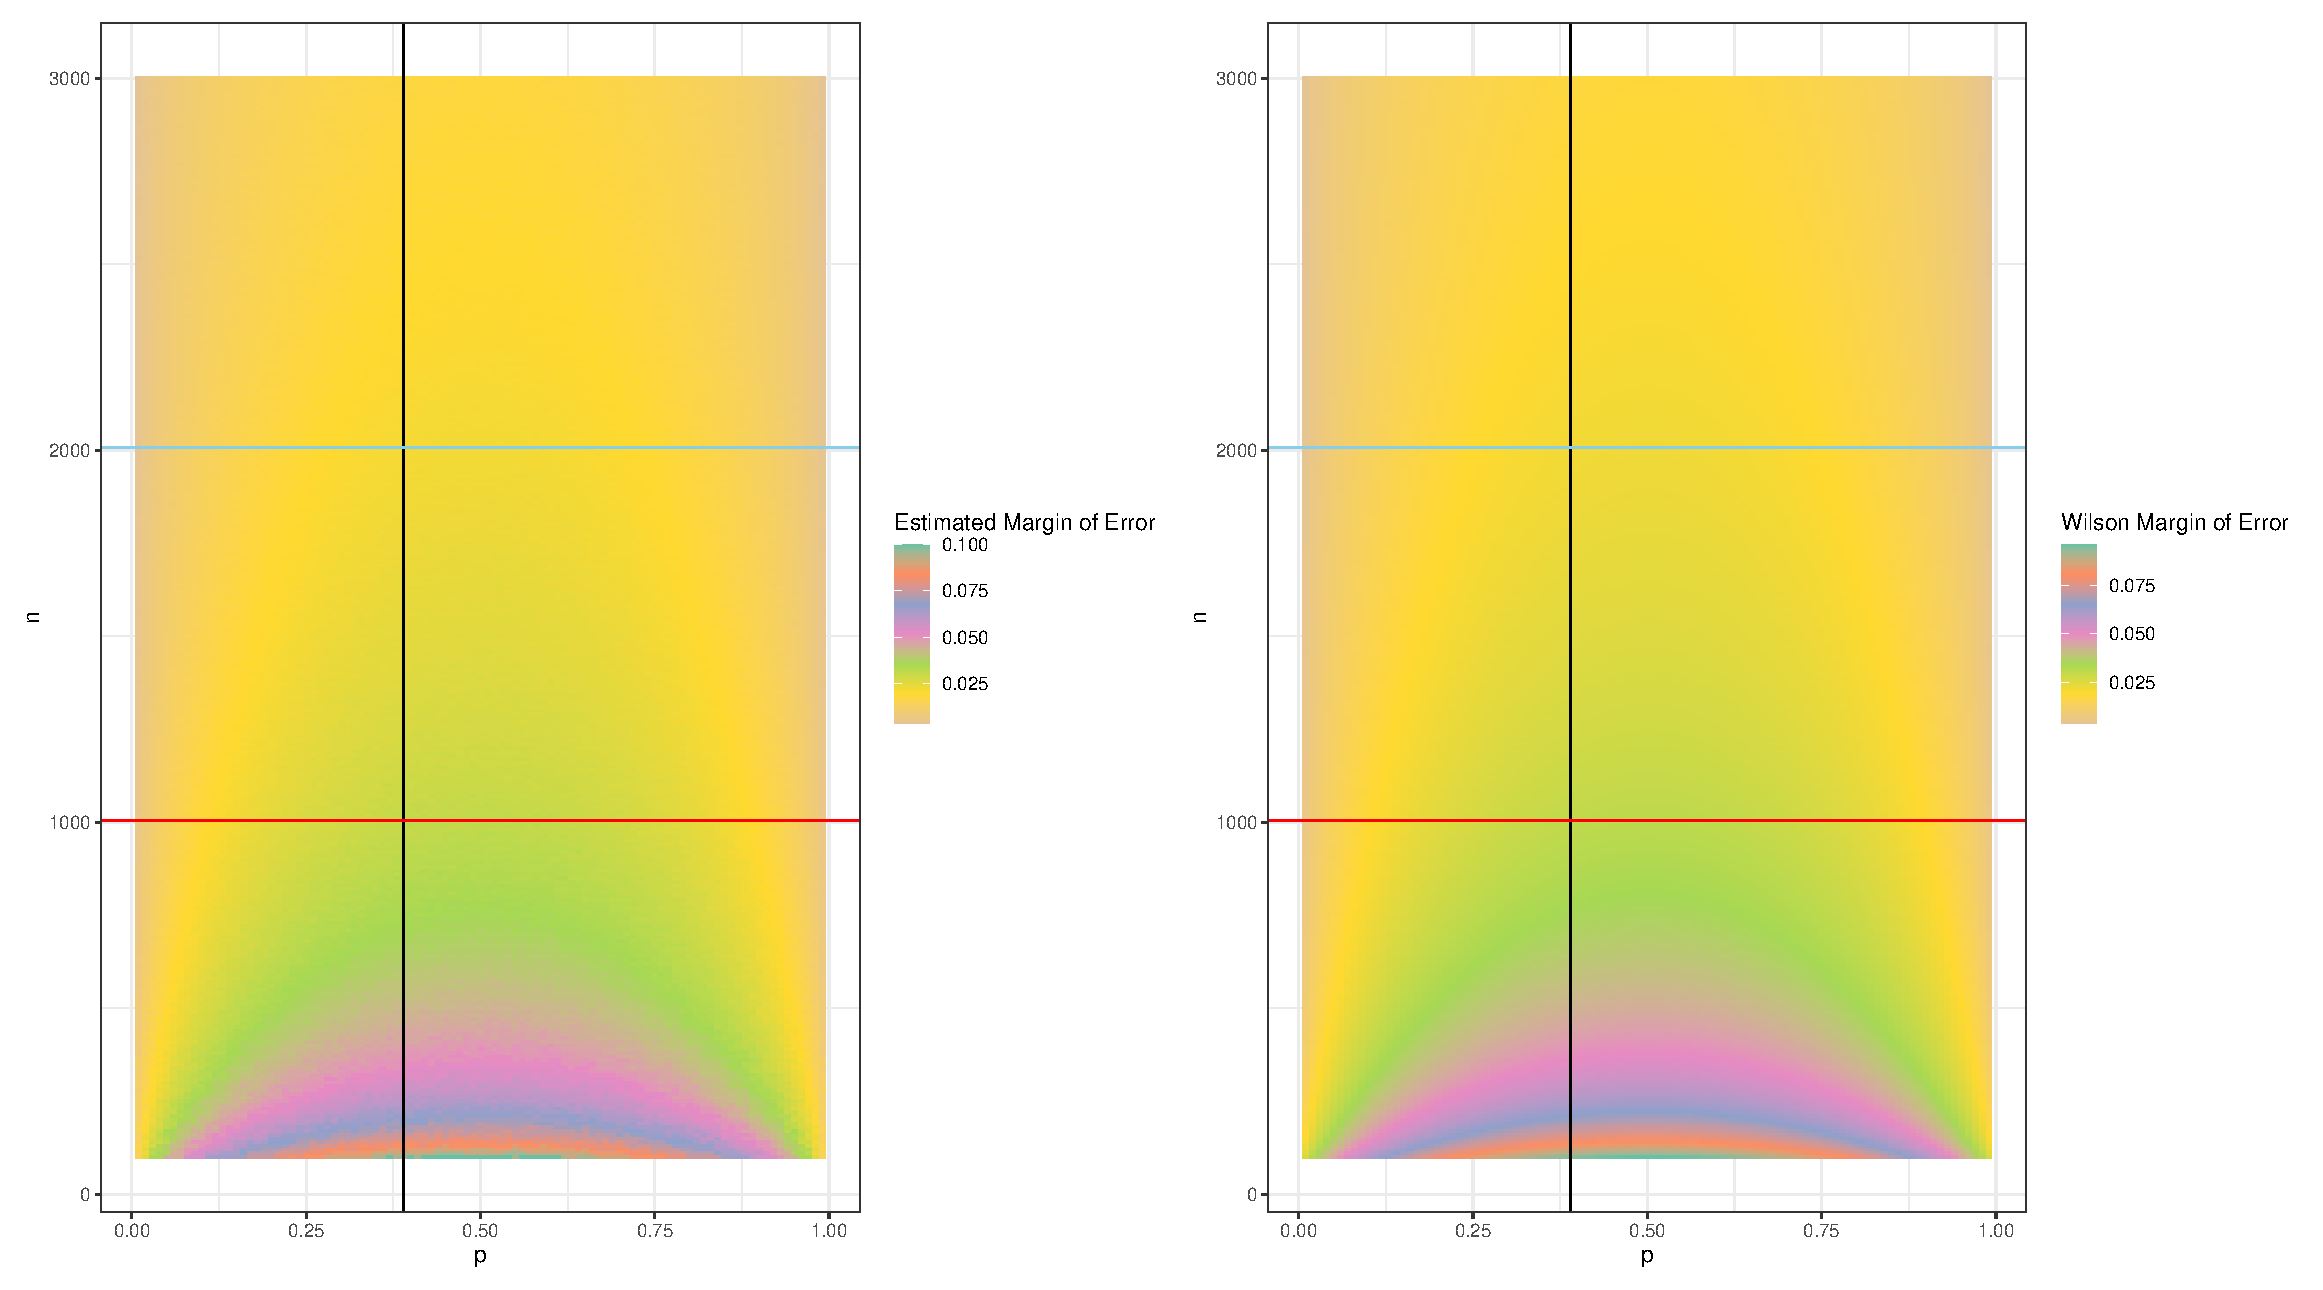
\includegraphics[scale=0.5]{Rplot02.pdf}
\captionof{figure}{Plots Showing The Realtionship Between MOE Values, n, and p}
\label{plot3}
\end{Figure}

\end{document}
